%%%%%%%%%%%%%%%%%%%%%%%%%%%%%%%%%%%%%%%%%%%%%%%%%%%%%%%%%%%%%%%%%%%%%%%%%%%%%%%%
%% Plantilla de memoria en LaTeX para la ETSIT - Universidad Rey Juan Carlos
%%
%% Por Gregorio Robles <grex arroba gsyc.urjc.es>
%%     Grupo de Sistemas y Comunicaciones
%%     Escuela T�cnica Superior de Ingenieros de Telecomunicaci�n
%%     Universidad Rey Juan Carlos
%% (muchas ideas tomadas de Internet, colegas del GSyC, antiguos alumnos...
%%  etc. Muchas gracias a todos)
%%
%% La �ltima versi�n de esta plantilla est� siempre disponible en:
%%     https://github.com/gregoriorobles/plantilla-memoria
%%
%% Para obtener PDF, ejecuta en la shell:
%%   make
%% (las im�genes deben ir en PNG o JPG)

%% Adaptado para la ETSII por Marcos Tenrero <tenrero@aol.com>

%%%%%%%%%%%%%%%%%%%%%%%%%%%%%%%%%%%%%%%%%%%%%%%%%%%%%%%%%%%%%%%%%%%%%%%%%%%%%%%%

\documentclass[a4paper, 12pt]{book}
%\usepackage[T1]{fontenc}

\usepackage[a4paper, left=2.5cm, right=2.5cm, top=3cm, bottom=3cm]{geometry}
\usepackage{times}
\usepackage[latin1]{inputenc}
\usepackage[spanish]{babel} % Comenta esta l�nea si tu memoria es en ingl�s
\usepackage{url}
%\usepackage[dvipdfm]{graphicx}
\usepackage{graphicx}
\usepackage[dvipsnames]{xcolor}
\usepackage{float}  %% H para posicionar figuras
\usepackage[nottoc, notlot, notlof, notindex]{tocbibind} %% Opciones de �ndice
\usepackage{listings} %% Bloques de c�digo
\usepackage{color} %% Paquete de color para listings
\usepackage{soul} %% Formato texto
\usepackage{dirtree} %% Tree de ficheros

\usepackage{glossaries}
\makeglossaries



\newcommand\YAMLcolonstyle{\color{red}\mdseries}
\newcommand\YAMLkeystyle{\color{black}\bfseries}
\newcommand\YAMLvaluestyle{\color{blue}\mdseries}

\makeatletter

% here is a macro expanding to the name of the language
% (handy if you decide to change it further down the road)
\newcommand\language@yaml{yaml}

\expandafter\expandafter\expandafter\lstdefinelanguage
\expandafter{\language@yaml}
{
  keywords={true,false,null,y,n},
  keywordstyle=\color{darkgray}\bfseries,
  basicstyle=\YAMLkeystyle,                                 % assuming a key comes first
  sensitive=false,
  comment=[l]{\#},
  morecomment=[s]{/*}{*/},
  commentstyle=\color{purple}\ttfamily,
  stringstyle=\YAMLvaluestyle\ttfamily,
  moredelim=[l][\color{orange}]{\&},
  moredelim=[l][\color{magenta}]{*},
  moredelim=**[il][\YAMLcolonstyle{:}\YAMLvaluestyle]{:},   % switch to value style at :
  morestring=[b]',
  morestring=[b]",
  literate =    {---}{{\ProcessThreeDashes}}3
                {>}{{\textcolor{red}\textgreater}}1     
                {|}{{\textcolor{red}\textbar}}1 
                {\ -\ }{{\mdseries\ -\ }}3,
}

% switch to key style at EOL
\lst@AddToHook{EveryLine}{\ifx\lst@language\language@yaml\YAMLkeystyle\fi}
\makeatother

\newcommand\ProcessThreeDashes{\llap{\color{cyan}\mdseries-{-}-}}


\graphicspath{ {./img/} }

\title{Memoria del Proyecto}
\author{Marcos Tenrero Mor�n}

\renewcommand{\baselinestretch}{1.5}  %% Interlineado

\begin{document}

\renewcommand{\refname}{Bibliograf�a}  %% Renombrando
\renewcommand{\appendixname}{Ap�ndice}

%%%%%%%%%%%%%%%%%%%%%%%%%%%%%%%%%%%%%%%%%%%%%%%%%%%%%%%%%%%%%%%%%%%%%%%%%%%%%%%%
% PORTADA

\begin{titlepage}
\begin{center}
\begin{tabular}[c]{c c}
%\includegraphics[bb=0 0 194 352, scale=0.25]{logo} &

\includegraphics[scale=0.25]{img/logo_vect.png} &
\begin{tabular}[b]{l}
\Huge
\textsf{UNIVERSIDAD} \\
\Huge
\textsf{REY JUAN CARLOS} \\
\end{tabular}
\\
\end{tabular}

\vspace{3cm}

\Large
GRADO EN INGENIER�A DE COMPUTADORES

\vspace{0.4cm}

\large
Curso Acad�mico 2017/2018

\vspace{0.8cm}

Trabajo Fin de Grado

\vspace{2.5cm}

\LARGE
DESPLIEGUE EL�STICO DE TESTS DE RENDIMIENTO

\vspace{4cm}

\large
Autor : Marcos Tenrero Mor�n \\
Tutor : Francisco Gort�zar
\end{center}
\end{titlepage}

\newpage
\mbox{}
\thispagestyle{empty} % para que no se numere esta pagina

%%%%%%%%%%%%%%%%%%%%%%%%%%%%%%%%%%%%%%%%%%%%%%%%%%%%%%%%%%%%%%%%%%%%%%%%%%%%%%%%
%%%% Dedicatoria

\chapter*{}
\pagenumbering{Roman} % para comenzar la numeracion de paginas en numeros romanos
\begin{flushright}
\textit{Dedicado a \\
mi familia / mi abuelo / mi abuela}
\end{flushright}

%%%%%%%%%%%%%%%%%%%%%%%%%%%%%%%%%%%%%%%%%%%%%%%%%%%%%%%%%%%%%%%%%%%%%%%%%%%%%%%%
%%%% Agradecimientos

\chapter*{Agradecimientos}
%\addcontentsline{toc}{chapter}{Agradecimientos} % si queremos que aparezca en el �ndice
\markboth{AGRADECIMIENTOS}{AGRADECIMIENTOS} % encabezado 


%%%%%%%%%%%%%%%%%%%%%%%%%%%%%%%%%%%%%%%%%%%%%%%%%%%%%%%%%%%%%%%%%%%%%%%%%%%%%%%%
%%%% Resumen

\chapter*{Resumen}
%\addcontentsline{toc}{chapter}{Resumen} % si queremos que aparezca en el �ndice
\markboth{RESUMEN}{RESUMEN} % encabezado

Aqu� viene un resumen del proyecto. Ha de constar de tres o cuatro p�rrafos, donde se presente de manera clara y concisa de qu� va el proyecto. 
Han de quedar respondidas las siguientes preguntas:

\begin{itemize}
  \item �De qu� va este proyecto? �Cu�l es su objetivo principal?
  \item �C�mo se ha realizado? �Qu� tecnolog�as est�n involucradas?
  \item �En qu� contexto se ha realizado el proyecto? �Es un proyecto
dentro de un marco general?
\end{itemize}

Lo mejor es escribir el resumen al final.

%%%%%%%%%%%%%%%%%%%%%%%%%%%%%%%%%%%%%%%%%%%%%%%%%%%%%%%%%%%%%%%%%%%%%%%%%%%%%%%%
%%%%%%%%%%%%%%%%%%%%%%%%%%%%%%%%%%%%%%%%%%%%%%%%%%%%%%%%%%%%%%%%%%%%%%%%%%%%%%%%
% �NDICES %
%%%%%%%%%%%%%%%%%%%%%%%%%%%%%%%%%%%%%%%%%%%%%%%%%%%%%%%%%%%%%%%%%%%%%%%%%%%%%%%%

% Las buenas noticias es que los �ndices se generan autom�ticamente.
% Lo �nico que tienes que hacer es elegir cu�les quieren que se generen,
% y comentar/descomentar esa instrucci�n de LaTeX.

%%%% �ndice de contenidos
\tableofcontents 
%%%% �ndice de figuras
\cleardoublepage
%\addcontentsline{toc}{chapter}{Lista de figuras} % para que aparezca en el indice de contenidos
\listoffigures % indice de figuras
%%%% �ndice de tablas
%\cleardoublepage
%\addcontentsline{toc}{chapter}{Lista de tablas} % para que aparezca en el indice de contenidos
%\listoftables % indice de tablas


%%%%%%%%%%%%%%%%%%%%%%%%%%%%%%%%%%%%%%%%%%%%%%%%%%%%%%%%%%%%%%%%%%%%%%%%%%%%%%%%
%%%%%%%%%%%%%%%%%%%%%%%%%%%%%%%%%%%%%%%%%%%%%%%%%%%%%%%%%%%%%%%%%%%%%%%%%%%%%%%%
% INTRODUCCI�N Y MOTIVACI�N %
%%%%%%%%%%%%%%%%%%%%%%%%%%%%%%%%%%%%%%%%%%%%%%%%%%%%%%%%%%%%%%%%%%%%%%%%%%%%%%%%

\cleardoublepage
\chapter{Introducci�n y Motivaci�n}
\label{sec:intro} % etiqueta para poder referenciar luego en el texto con ~\ref{sec:intro}
\pagenumbering{arabic} % para empezar la numeraci�n de p�gina con n�meros

La �ltima era de la inform�tica no ha parado de evolucionar durante las �ltimas d�cadas, han surgido y se han puesto en pr�ctica diversas metodolog�as en el desarrollo del software, desde el modelo de procesos hasta las m�s actuales como las denominadas metodolog�as �giles, formadas por una serie de t�cnicas y de m�todos como Extreme Programming , Kanban o Scrum.

En la actualidad, el uso de las metodolog�as �giles est� en auge, y esto conlleva la adopci�n de una nueva manera de concebir la inform�tica, dando prioridad a fases que antes no se ten�an en cuenta, como es el caso de la fase de testing.

En el mundo del desarrollo del software, el testing, es quiz�s, una de las partes m�s importantes del ciclo, ya que permiten asegurar la estabilidad del producto entre las diferentes iteraciones del desarrollo.  

Dentro de esta etapa, existen diversos tipos de pruebas a realizar, pero este trabajo de fin de grado se centra  en las pruebas de rendimiento.

En t�rminos de calidad de software, a la hora de realizar un test, se tiene muy en cuenta la pir�mide de test, la cual pretende dar unas gu�as generales a tener en cuenta con respecto a la cantidad de test que se deber�an desarrollar para un proyecto, teniendo en cuenta su complejidad de codificaci�n y mantenimiento.

Normalmente se sit�an en la cima esta pir�mide los tests de sistema o End-To-End (\gls{E2E}) ya que el coste de �stos es muy elevado al requerir que todos los componentes de la aplicaci�n se encuentren operativos en el momento de realizaci�n de las pruebas y al ser m�s fr�giles. Los test de rendimiento se encuentran justo en esta cima.  

El an�lisis del rendimiento de una aplicaci�n es crucial para poder comprobar que �sta escala de una manera apropiada con diferentes cargas de trabajo. Normalmente, es un aspecto que se suele olvidar en las etapas iniciales del desarrollo, ya que es un factor que suele preocupar m�s en aplicaciones que ya tienen una carga considerable.

No s�lo es una etapa relegada debido a que no suele ser un factor preocupante en las primeras iteraciones del desarrollo, sino que tambi�n resulta complicado el establecer una infraestructura para poder ejecutar, y sobre todo, mantener este tipo de tests.


Este trabajo cubre el desarrollo de una herramienta que ayude en el proceso del an�lisis de rendimiento de cualquier aplicaci�n. Pretende ofrecer una manera sencilla de ejecutar estos test de manera autom�tica y distribuida sin tener que preocuparse de la infraestructura subyacente necesaria, ya que normalmente, con los test de rendimiento se pretende simular una gran carga de trabajo sobre la aplicaci�n y esto se traduce en muchas conexiones simult�neas a la misma, y para ello, se necesitan diversos nodos para poder distribuir esta simulaci�n de la carga. 


\clearpage

La parte mas tediosa de trabajar con diversos nodos es la configuraci�n de �stos para que est�n preparados para realizar su cometido. 

Por ello, para una efectiva gesti�n, es necesario poder desplegar y ejecutar estos tests de manera sencilla, y la �nica manera de hacerlo �gilmente, es contemplar el paradigma de cloud computing, que aporta el concepto de contenedores y un despliegue r�pido de infraestructura bajo demanda.

La herramienta que se ha desarrollado durante la realizaci�n de este trabajo de fin de grado a�ade una capa de abstracci�n a la tecnolog�a de orquestaci�n de contenedores por excelencia, Docker. Lo que se traduce en la posibilidad de ejecutar cualquier tipo de aplicaci�n que requiera este modelo de despliegue, aunque como ejemplo, se ha tomado como referencia la herramienta Apache JMeter.

Por otra parte, llevo cerca de dos a�os trabajando en el departamento de automatizaci�n y calidad de software en una empresa multinacional de desarrollo de software, estando estos valores y premisas muy presentes en mi vida laboral. En los �ltimos meses, el an�lisis de rendimiento ha sido un objetivo muy importante en esta empresa, y mi labor se ha centrado en gran medida en esta tarea, dise�ando y desplegando toda la infraestructura necesaria para poner en pr�ctica el proyecto. 

Este hecho me ha permitido probar en primera l�nea los avances sobre mi trabajo de fin de grado en un entorno empresarial real. 

\section{Despliegue tradicional de Apache JMeter}

Apache JMeter tiene diversos modos de funcionamiento, ya que ofrece dos interfaces, una gr�fica y otra por l�nea de comandos. Para aprovechar varios nodos y poder lanzar un test de carga de forma distribuida, es necesario ejecutar la aplicaci�n en modo esclavo en cada uno de los nodos remotos en los que se va a ejecutar el test.\newline

Por otro lado, estos nodos deben estar visibles entre s� dentro de la red, lo que implica una configuraci�n manual del firewall para poder as� abrir los puertos necesarios.\newline

Un despliegue t�pico consistir�a en los siguientes pasos:

\subsubsection{Descarga de Apache JMeter}
Bien via repositorio de paquetes \textit{Debian} o \textit{Red-Hat based} o v�a fichero comprimido con los binarios pre-compilados por la fundaci�n Apache.\newline

Como ejemplo se va usar una distribuci�n CentOS 7, basada en RedHat utilizando los binarios disponibles desde la p�gina oficial de JMeter.

\begin{lstlisting}[language=bash]
  $ wget https://archive.apache.org/dist/jmeter/binaries/ \
  apache-jmeter-3.3.zip
  $ unzip jmeter-3.3.zip
\end{lstlisting}  

Con estos comandos se dispondr�a de los binarios de JMeter preparados para ser ejecutados en pr�cticamente cualquier sistema UNIX.

\subsubsection{Configuraci�n del firewall}

JMeter requiere que el firewall est� correctamente configurado para permitir la comunicaci�n entre nodos, esto implica la apertura de diversos puertos como \textbf{1099},\textbf{1664} entre otros, ya que depende de la configuraci�n que se realice sobre JMeter. 

Dependiendo de la distribuci�n sobre la que realizar las configuraciones, se usar� un comando u otro, los m�s t�picos son los siguientes:

\textbf{Ubuntu UFW}

\begin{lstlisting}[language=bash]
  $ ufw allow <port>/tcp
\end{lstlisting}

\textbf{IP Tables}

\begin{lstlisting}[language=bash]
  $ iptables -A INPUT -p tcp --dport <port> -j ACCEPT
\end{lstlisting}

\textbf{Firewall-cmd}

\begin{lstlisting}[language=bash]
  $ firewall-cmd --zone=public --add-port=<port>/tcp --permanent
\end{lstlisting}

Tratar con la complejidad de la configuraci�n del firewall y de la red se vuelve realmente complejo y m�s cuando se dispone de una gran cantidad de nodos y �stos son heterog�neos en lo que a Sistema Operativo se refiere.

\subsubsection{Despliegue de esclavos}

Apache JMeter requiere de un orden de arranque espec�fico, primero deben arrancarse los nodos esclavos con el siguiente comando:

\begin{lstlisting}[language=bash]
  $ ./jmeter-server -Dserver.rmi.localport=4445 -Dserver_port=1099 
\end{lstlisting}

Este comando debe ser ejecutado en cada uno de los nodos que vayan a ser empleados como esclavos. 

\subsubsection{Arranque del nodo Maestro}

Es necesario manejar y actualizar constantemente la lista de las direcciones de los nodos a los que que conectarse a trav�s del nodo maestro para ejecutar un test de carga distribuido ya que es necesario especificar expl�citamente los nodos remotos.\newline

Para ejecutar un test de carga distribuido, una vez que la infraestructura previa est� correctamente configurada, basta con ejecutar un comando similar al siguiente:

\begin{lstlisting}[language=bash]
  $ ./jmeter -n -t $TEST_PATH -R$REMOTES -Dserver.rmi.localport=60000 
\end{lstlisting}

\subsubsection{Publicaci�n de resultados}

Es posible especificar un \textbf{\textit{Listener}} durante la ejecuci�n del nodo maestro junto al test para as� poder exportar en tiempo real los resultados del test a un sistema externo como \textit{Apache Kafka}, \textit{ElasticSearch}, una base de datos entre otros.

\subsubsection{Consideraciones adicionales: Cifrado de comunicaciones}

Es com�n utilizar un cifrado \gls{SSL} o \gls{TLS} en las comunicaciones de red, y JMeter permite encriptar las comunicaciones entre los diferentes nodos con SSL\footnote{https://jmeter.apache.org/usermanual/remote-test.html\#setup\_ssl}. Esto requiere de la generaci�n de certificados y de un almac�n de claves, lo que dificulta, aun mas, el despliegue de un cl�ster de forma tradicional.


%%%%%%%%%%%%%%%%%%%%%%%%%%%%%%%%%%%%%%%%%%%%%%%%%%%%%%%%%%%%%%%%%%%%%%%%%%%%%%%%
%%%%%%%%%%%%%%%%%%%%%%%%%%%%%%%%%%%%%%%%%%%%%%%%%%%%%%%%%%%%%%%%%%%%%%%%%%%%%%%%
% OBJETIVOS %
%%%%%%%%%%%%%%%%%%%%%%%%%%%%%%%%%%%%%%%%%%%%%%%%%%%%%%%%%%%%%%%%%%%%%%%%%%%%%%%%

\cleardoublepage % empezamos en p�gina impar
\chapter{Objetivos} % t�tulo del cap�tulo (se muestra)
\label{chap:objetivos} % identificador del cap�tulo (no se muestra, es para poder referenciarlo)

1 p�gina describiendo los objetivos concretos que se pretenden conseguir con el desarrollo del proyecto. Es como la conclusi�n del cap�tulo anterior.


%%%%%%%%%%%%%%%%%%%%%%%%%%%%%%%%%%%%%%%%%%%%%%%%%%%%%%%%%%%%%%%%%%%%%%%%%%%%%%%%
%%%%%%%%%%%%%%%%%%%%%%%%%%%%%%%%%%%%%%%%%%%%%%%%%%%%%%%%%%%%%%%%%%%%%%%%%%%%%%%%
% TECNOLOG�AS Y HERRAMIENTAS %
%%%%%%%%%%%%%%%%%%%%%%%%%%%%%%%%%%%%%%%%%%%%%%%%%%%%%%%%%%%%%%%%%%%%%%%%%%%%%%%%

\cleardoublepage
\chapter{Metodolog�as}

Este proyecto ha seguido la filosof�a de las metodolog�as �giles, es decir, un desarrollo e incremental.\newline

Dado el car�cter din�mico de la disponibilidad del tiempo, se ha optado por una planificaci�n \textbf{Kanban}, una vez definidos los requisitos y plan de acci�n del proyecto.\newline

Adem�s ha sido vital afrontar la filosof�a DevOps, aplicando desde el comienzo del proyecto la integraci�n continua, para asegurar la salud del producto con cada nueva iteraci�n, ya que al trabajar directamente con la API del demonio de Docker, cualquier m�nimo cambio afectaba al resto del proyecto.

\section{Extreme Programming}

Extreme Programming es una pr�ctica bastante extendida en el mundo del desarrollo de software. Obliga a definir la estructura del c�digo e incluso los tests antes de desarrollar el producto final, de tal manera, en primer lugar se dise�an y se implementan los tests, los cuales fallar�n hasta que la funcionalidad est� implementada completamente.\newline

Esta metodolog�a obliga al programador a pensar en el dise�o en un primer lugar, dotando al software de mas calidad.

\section{Kanban}

Kanban es un modelo �gil de organizaci�n del desarrollo de software que se caracteriza en la divisi�n de las tareas en diferentes estados, t�picamente, \textit{PENDIENTE}, \textit{EN PROGRESO} y \textit{TERMINADO}. \newline

Se ha utilizado la gesti�n de proyectos en el propio repositorio que ofrece la plataforma GitHub\footnote{https://github.com/mtenrero/ATQ-Director/projects/1} para que estuviese disponible para la comunidad de forma sencilla. Adem�s ofrece sincronizaci�n autom�tica de tareas basada en \textit{Issues} y \textit{Pull Requests}.\newline


\begin{figure}[h]
    \centering
    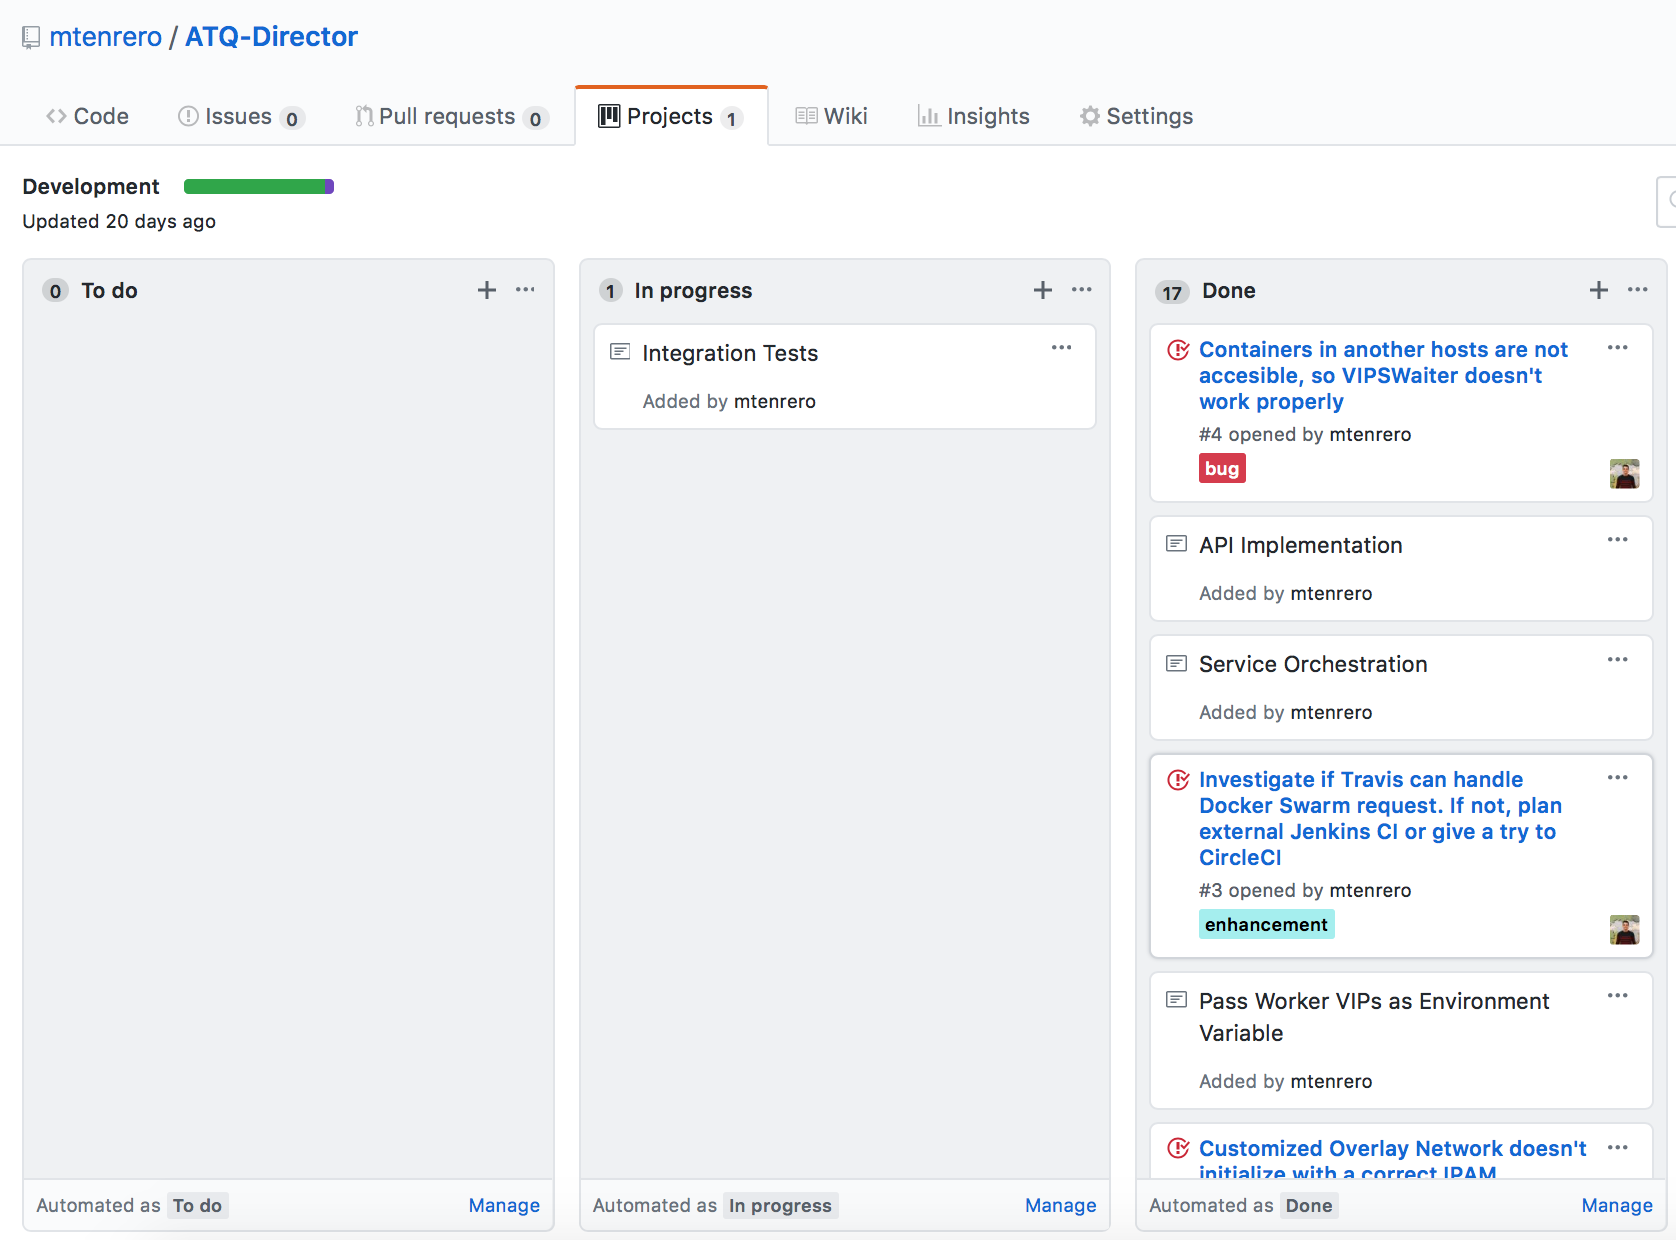
\includegraphics[width=1\textwidth]{kanban-github}
    \caption{Tablero Kanban del proyecto en GitHub}
    \label{fig:kanban}
\end{figure}


%%%%%%%%%%%%%%%%%%%%%%%%%%%%%%%%%%%%%%%%%%%%%%%%%%%%%%%%%%%%%%%%%%%%%%%%%%%%%%%%
%%%%%%%%%%%%%%%%%%%%%%%%%%%%%%%%%%%%%%%%%%%%%%%%%%%%%%%%%%%%%%%%%%%%%%%%%%%%%%%%
% TECNOLOG�AS Y HERRAMIENTAS %
%%%%%%%%%%%%%%%%%%%%%%%%%%%%%%%%%%%%%%%%%%%%%%%%%%%%%%%%%%%%%%%%%%%%%%%%%%%%%%%%

\cleardoublepage
\chapter{Tecnolog�as, Herramientas y Metodolog�as}

Aqu� me gustar�a hablar de los siguientes temas:



\begin{enumerate}
  \item \textbf{Lenguaje Golang:} Car�cteristicas b�sicas del lenguaje, cross-platform, cobertura de test
  \item \textbf{Git, Travis \& Jenkins:} Diferencias y features cr�ticas que me han hecho pasar de Travis a Jenkins
  \item \textbf{Swagger:}
  \item \textbf{Goa Design:} Paquete Golang, Design First API, creo que es importante por el car�cter de piensa antes de picar, muy similar a TDD
  \item \textbf{AWS} Toda la CI est� desplegada en AWS y tengo pensado montar un cluster Swarm aqu� para una futura demo.
  \item \textbf{Docker}
  \item \textbf{ElasticSearch} Caracter�sticas b�sicas
  \item \textbf{Shared Filesystem:} GlusterFS / Samba . No es Kubernetes, asi que se necesita esta configuraci�n previa para tener todos los ficheros disponibles en todo el cluster. Explicar lo que ofrece y por qu� es necesario.
  \item \textbf{Redes:} Concretamente DNS y algoritmo DNS Round Robin. Es la piedra angular en cuanto a orquestaci�n con arquitectura Master / Workers se refiere
  \item \textbf{Apache Jmeter:} Forma de ejecuci�n distribuida y arquitectura
\end{enumerate}

\section{Golang}

Go es un lenguaje de programaci�n que se comenz� a desarrollar en 2007 \cite{Pike:2012:GG:2384716.2384720} y naci� con el ideal de eliminar todos los obst�culos de la programaci�n actual \cite{donovan2015go}, ya que desde hace varios a�os no hab�a salido ning�n lenguaje de programaci�n de alta importancia. Se necesitaba que estuviese dise�ado por completo, teniendo en cuenta factores de la inform�tica actual, como la concurrencia o la rapidez en la compilaci�n y en la codificaci�n.

Los or�genes de Go se remontan a los lenguajes Oberon 2 , C y Alef \cite{donovan2015go}. Nace como un proyecto de Google como soluci�n para la codificaci�n de soluciones complejas.

Como particular caracter�stica \cite{pike2009go}, Go es un lenguaje de programaci�n con recolector de basura, para permitir as� trabajar de una forma correcta con la concurrencia de las aplicaciones. \newline

 El compilador de Go se ide� de tal forma para que fuese compatible nativamente con todos los Sistemas Operativos, introduciendo el cross-compile (Compilaci�n para otras plataformas o arquitecturas en un �nico Sistema Operativo) como uno de sus puntos fuertes.
 
\section{Dep: Go Dependency Management}

Uno de los puntos fuertes de Go, es la gesti�n de dependencias durante la compilaci�n \cite{pike2009go}. Sin embargo, de cara al desarrollador, por defecto, carece de un fichero a nivel global de proyecto para poder definir las dependencias del mismo y/o la versi�n con la que se desea trabajar, sino que se debe especificar a trav�s de sentencias \textit{import} en los ficheros \textit{.go} del c�digo. Adem�s, para poder usar esas dependencias, es necesario que est�n presentes en el \$GOPATH del sistema.\newline

Dep nace como un experimento de Golang\footnote{https://github.com/golang/dep} , preparada para usar en producci�n, aunque sin llegar a ser la herramienta oficial de gesti�n de dependencias a nivel de proyecto/usuario. Emplea un fichero TOML en la raiz del proyecto, en �l se indica la dependencia requerida, su versi�n e incluso la rama del control de versiones desde la cual obtener los paquetes. \newline

\section{Goa Design: Design-first Network framework}

Goa\footnote{https://goa.design} es un framework completo para construir microservicios en Go que invierte la forma de construir APIs web completamente. Posee generaci�n autom�tica de c�digo y documentaci�n. \newline

Es un framework enfocado al dise�o de la API en primer lugar, y es lo que hace a este framework �nico. Posee su propio lenguaje DSL (lenguaje descriptivo) en el que antes de codificar, obliga al programador a pensar en el dise�o de la API, ya que esta debe ser definida en un primer lugar. Permite definir desde el endpoint, el contenido que consumir� y los par�metros que recibir�.

\section{OpenAPI Specification}

OpenAPI es una especificaci�n mantenida e ideada por la comunidad Open-Source en la plataforma GitHub\footnote{https://github.com/OAI/OpenAPI-Specification}, independiente de cualquier lenguaje de programaci�n, que permite definir cualquier tipo con toda la especificaci�n completa de una API, para que sea comprensible, tanto para personas como para ordenadores, ya que se basa en ficheros JSON y YAML.

\section{DNS}

Domain Name System es un sistema de nombrado de redes IP que se utiliza para resolver nombres en direcciones IP. El servicio de resoluci�n de nombres puede tener diferentes tipos de registros. En la investigaci�n del trabajo s�lo se han usado registros de tipo \textbf{A}, los cuales traducen un nombre en una o varias direcciones IP, dependiendo de los registros A que tenga almacenados para un mismo nombre de dominio/subdominio.

\subsection{DNS Round-Robin}

DNS Round-Robin es un algoritmo de selecci�n de IP, en el que con cada petici�n que realiza el usuario, se obtiene una lista completa de todas las direcciones IP registradas en el servidor de nombres ordenada de tal forma que nunca recibe la misma IP, realizando, de esta manera, labores de balanceador de carga.

Docker implementa este algoritmo de forma alternativa en su DNS interno, y el desarrollador puede elegir si desea operar con DNS Round Robin o con \textit{Routing Mesh}, balanceo de carga interno, donde el nombre es resuelto con una �nica IP Virtual de manera no determinista.\newline

Cuando se opta por usar el modo DNS Round-Robin, por limitaciones de dise�o, resulta imposible exponer puertos hacia el host, �nicamente se permiten conexiones de red con las redes indicadas por el servicio. 

\section{Contenedores}

Los contenedores son un nuevo tipo de virtualizaci�n ligera de Sistemas Operativos que no requieren la emulaci�n de instrucciones en el procesador, reduciendo as� el consumo de recursos sin prescindir del aislamiento necesario presente en la virtualizaci�n tradicional \cite{containerVsHyper}.

\subsection{LXC: Linux Containers}

LXC es un tipo de virtualizaci�n basada en contenedores, usa el espacio de nombres de kernel y cgroups para asegurar el aislamiento de los contenedores, aunque los contenedores comparten el kernel con el Sistema Operativo del host \cite{ContainersComparison}.

\subsection{Docker}

Docker a�ade una capa para gestionar las redes de los contenedores dot�ndolos de una IP propia y el sistema de ficheros a LXC. Permite especificar im�genes de contenedores autocontenidas y gestionar el ciclo de vida de ellos. 
\cite{containerVsHyper} \cite{fromLXCtoKubernetes}. Introduce un modelo cliente-servidor, siendo el demonio de Docker en el host el responsable de la comunicaci�n con los contenedores \cite{ContainersComparison} \newline 

Docker ofrece adem�s un repositorio o registro donde almacenar estas im�genes de los contenedores para que est�n disponibles para su uso
\cite{Merkel:2014:DLL:2600239.2600241}
de manera p�blica a trav�s de DockerHub\footnote{https://hub.docker.com}, o de manera privada con un registro desplegado a demanda.

Docker usa una terminolog�a propia:

\begin{itemize}
  \item \textbf{Imagen:} Descripci�n de los contenidos de un contenedor, interoperable entre todo el ecosistema Docker.
  \item \textbf{Contenedor:} Es la unidad m�nima en Docker, corresponde a una imagen ejecutada sobre una m�quina o Swarm.
  \item \textbf{Volumen:} Unidad de almacenamiento persistente en Docker, pueden ser bindados a un directorio o fichero del sistema de ficheros del host o en el propio contexto de Docker.
  \item \textbf{Servicio:} Encapsulaci�n de una imagen que se puede configurar de manera concreta. Permitiendo configurar la cantidad de replicas a desplegar, el tipo de red o los vol�menes con los que trabajar.
  \item \textbf{Red:} Red dentro del ecosistema Docker, se encarga de interconectar Servicios y/o Contenedores
\end{itemize}


\subsubsection{Raft Consensus}

Es un algoritmo para asegurar tolerancia a fallos. Para su correcto funcionamiento, se tiene que establecer un \textit{Quorum}, un conjunto de nodos elegidos para administraci�n. El tama�o del \textit{Quorum} se define por la siguiente ecuaci�n \( 2f + 1 \), siendo \( f \) la cantidad de fallos a tolerar. Por lo tanto, para formar \textit{Quroum}, ser�n necesarios un m�nimo de 3 nodos \cite{Raft-UCAM-CL-TR-857} .

\subsubsection{Docker Swarm}

Docker Swarm es un modo de funcionamiento de Docker que permite utilizar diversas m�quinas para formar un cl�ster de Docker en el que desplegar contenedores, donde el demonio de Docker gestiona la red, el sistema de ficheros y la comunicaci�n entre servicios.\newline

Para desplegar diversos Servicios en un Swarm, Docker introduce el concepto de \textbf{Stack}, una agrupaci�n de Servicios con su configuraci�n de red particular.\newline 

Los nodos de Docker Swarm pueden tener dos roles:

\begin{itemize}
  \item \textbf{Manager:} Gestionan el cl�ster, como m�nimo, debe haber 3 Managers para que se puede aplicar Raft-Consensus. Tienen una visi�n completa del cluster. A su vez, uno de ellos se elegir� como \textbf{L�der}, el cual ser� responsable de la gesti�n del cl�ster. 
  \item \textbf{Worker:} Son nodos en los cuales s�lo se despliegan contenedores o servicios, s�lo tienen visi�n de los contenedores o servicios que est�n desplegados en el propio nodo.
\end{itemize}



%%%%%%%%%%%%%%%%%%%%%%%%%%%%%%%%%%%%%%%%%%%%%%%%%%%%%%%%%%%%%%%%%%%%%%%%%%%%%%%%
%%%%%%%%%%%%%%%%%%%%%%%%%%%%%%%%%%%%%%%%%%%%%%%%%%%%%%%%%%%%%%%%%%%%%%%%%%%%%%%%
% DESCRIPCI�N INFORM�TICA %
%%%%%%%%%%%%%%%%%%%%%%%%%%%%%%%%%%%%%%%%%%%%%%%%%%%%%%%%%%%%%%%%%%%%%%%%%%%%%%%%

\cleardoublepage
\chapter{Descripci�n inform�tica}


\section{Requisitos}
\label{sec:requisitos}

Descripci�n m�s detallada de los objetivos explicados en el cap�tulo de Objetivos

Tareas tablero Kanban del Project de GitHub

\section{Arquitectura y An�lisis}
\label{sec:arquitectura-analisis}

Como el "orquestador" se ha centrado en el formato de despliegue Master/Workers, explicaci�n de la forma de ejecuci�n de JMeter en detalle

Explicaci�n de la investigaci�n hasta que di con la forma de orquestar los servicios de manera satisfactoria para nuestro objetivo siguiendo los requisitos de JMeter.

Arquitectura inicial, con alg�n boceto de arquitectura.

Docker Swarm Architecture + GlusterFS

\section{Dise�o e Implementaci�n}
\label{sec:diseno-implementacion}

\begin{itemize}
  \item Diagrama de estados del proceso de orquestaci�n
  \item Dise�o de la API REST, funciones, endpoints...
  \item Dockerfile JMeter con su script bash
  \item Dockerfile build Golang + dep dependency manager
  \item Implementaci�n algoritmo Descubrimiento de contenedores DNSRR
\end{itemize}




\section{Pruebas}
\label{sec:pruebas}

Hablar de Cobertura de Test, como se ha organizado por paquetes, c�mo est� integrado con el Pipeline de IC de Jenkins, los triggers que tiene configurado... 
\newline

Explicar c�mo se dise�aron primero los tests b�sicos, luego la implementaci�n, y despu�s se ampli� la cobertura de tests



%%%%%%%%%%%%%%%%%%%%%%%%%%%%%%%%%%%%%%%%%%%%%%%%%%%%%%%%%%%%%%%%%%%%%%%%%%%%%%%%
%%%%%%%%%%%%%%%%%%%%%%%%%%%%%%%%%%%%%%%%%%%%%%%%%%%%%%%%%%%%%%%%%%%%%%%%%%%%%%%%
% CONCLUSIONES Y TRABAJOS FUTUROS%
%%%%%%%%%%%%%%%%%%%%%%%%%%%%%%%%%%%%%%%%%%%%%%%%%%%%%%%%%%%%%%%%%%%%%%%%%%%%%%%%

\cleardoublepage
\chapter{Conclusiones y trabajos futuros}
\label{chap:conclusiones-trabajos-futuros}

Me gustar�a hablar de la integraci�n completa con OS Windows, otros tipos de despliegue como en AWS de manera nativa, otros modelos diferentes a la arquitectura Master/Workers...

Quiz�s de una interfaz web completa con Angular o similar... 


%%%%%%%%%%%%%%%%%%%%%%%%%%%%%%%%%%%%%%%%%%%%%%%%%%%%%%%%%%%%%%%%%%%%%%%%%%%%%%%%
%%%%%%%%%%%%%%%%%%%%%%%%%%%%%%%%%%%%%%%%%%%%%%%%%%%%%%%%%%%%%%%%%%%%%%%%%%%%%%%%
% BIBLIOGRAFIA %
%%%%%%%%%%%%%%%%%%%%%%%%%%%%%%%%%%%%%%%%%%%%%%%%%%%%%%%%%%%%%%%%%%%%%%%%%%%%%%%%

\cleardoublepage

% Las siguientes dos instrucciones es todo lo que necesitas
% para incluir las citas en la memoria
\bibliographystyle{abbrv}
\bibliography{memoria}  % memoria.bib es el nombre del fichero que contiene
% las referencias bibliogr�ficas. Abre ese fichero y mira el formato que tiene,
% que se conoce como BibTeX. Hay muchos sitios que exportan referencias en
% formato BibTeX. Prueba a buscar en http://scholar.google.com por referencias
% y ver�s que lo puedes hacer de manera sencilla.
% M�s informaci�n: 
% http://texblog.org/2014/04/22/using-google-scholar-to-download-bibtex-citations



%%%%%%%%%%%%%%%%%%%%%%%%%%%%%%%%%%%%%%%%%%%%%%%%%%%%%%%%%%%%%%%%%%%%%%%%%%%%%%%%
%%%%%%%%%%%%%%%%%%%%%%%%%%%%%%%%%%%%%%%%%%%%%%%%%%%%%%%%%%%%%%%%%%%%%%%%%%%%%%%%
% AP�NDICE(S) %
%%%%%%%%%%%%%%%%%%%%%%%%%%%%%%%%%%%%%%%%%%%%%%%%%%%%%%%%%%%%%%%%%%%%%%%%%%%%%%%%
\newacronym{LDAP}{LDAP}{Lightweight Directory Access Protocol}

\newacronym{ATQ}{ATQ}{Automation Test Queue}

\newacronym{ELK}{ELK}{Elastic + Logstash + Kibana}

\newacronym{API}{API}{Interfaz de Programaci�n de Aplicaciones}

\newacronym{E2E}{E2E}{End to End}

\newacronym{SSL}{SSL}{Secure Sockets Layer}

\newacronym{TLS}{TLS}{Transport Layer Security}

\newacronym{SAAS}{SAAS}{Software As A Service}

\newacronym{PAAS}{PAAS}{Platform As A Service}

\newacronym{DSL}{DSL}{Lenguaje de Dominio Espec�fico}

\newacronym{DNS}{DNS}{Domain Name System}

\newacronym{FS}{FS}{FileSystem, Sistema de ficheros}

\newacronym{CI}{CI}{Continuous Integration}

\newacronym{CD}{CD}{Continuous Deployment}

\newacronym{SDK}{SDK}{Software Development Kit}

\newacronym{CSV}{CSV}{Valores separados por comas}

\newacronym{WIP}{WIP}{Work In Progress}

\newacronym{HTTP}{HTTP}{Hypertext Transfer Protocol}

\newacronym{EC2}{EC2}{Instancia virtual de Amazon Web Services}

\newacronym{AWS}{AWS}{Amazon Web Services}

\newacronym{TDD}{TDD}{Test\-Driven\-Development}

\newacronym{REST}{REST}{Representational State Transfer}

\newacronym{UUID}{UUID}{Identificador �nico}

\cleardoublepage
%Print the glossary
\printglossaries

\cleardoublepage
\appendix
\chapter{Manual de usuario}
\label{app:manual}

\appendixname{b}
\chapter{Im�genes Docker}
\label{code-snippets}

\definecolor{pblue}{rgb}{0.13,0.13,1}
\definecolor{pgreen}{rgb}{0,0.5,0}
\definecolor{pred}{rgb}{0.9,0,0}
\definecolor{pgrey}{rgb}{0.46,0.45,0.48}

\lstset{language=yaml,
  showspaces=false,
  showtabs=false,
  breaklines=true,
  showstringspaces=false,
  breakatwhitespace=true,
  commentstyle=\color{pgreen},
  keywordstyle=\color{pblue},
  stringstyle=\color{pred},
  basicstyle=\small,
  moredelim=[il][\textcolor{pgrey}]{$$},
  moredelim=[is][\textcolor{pgrey}]{\%\%}{\%\%}
}

\begin{lstlisting}[language=yaml, caption=ATQ docker-compose.yaml]
version: 3.3

services:
    atq:
        image: tenrero/atq
        tty: true
        volumes:
            - gluster:/gluster:rw
            - /var/run/docker.sock:/var/run/docker.sock
        ports:
            - "8080:8080"
        deployment:
            mode: global
            placement:
                constraints: [node.role == manager]
volumes:
    gluster:

\end{lstlisting}

\clearpage

\begin{lstlisting}[caption=ATQ Dockerfile]
\end{lstlisting}
FROM centos

LABEL MAINTAINER="Marcos Tenrero"

COPY ./releases/atq-director-linux-amd64 /atq/atq-amd64
COPY controller-config.docker.yaml /controller-config.yaml

RUN mkdir -p /gluster/storage

EXPOSE 8080

RUN cd /atq

ENTRYPOINT [ "/atq/atq-amd64" ]
\end{document}
